\chapter{Introduction} 
\label{chapter:introduction}

\begin{introduction}
    "The only source of knowledge is experience." - Albert Einstein
\end{introduction}



\section{Internship Context and Framework} \label{sec:intro_context}

This document represents the final report of the internship carried out as part of the Internship Curricular Unit (49991) of the second year of studies of the Master's Degree in Clinical Bioinformatics, with specialization in Genome Bioinformatics, at the University of Aveiro. The internship lasted nine months, starting on November 21st, 2023, and ending on July 19th, 2024, totalling 1296 hours of work. 

During this period, the trainee had the opportunity to apply the knowledge acquired throughout the course and to get involved in practical projects related to bioinformatics and genomics. Unilabs, a recognized company in the health area, provided a professional environment where the intern could collaborate with experienced professionals and actively participate in projects relevant to clinical bioinformatics. This report addresses the activities developed during the internship and the contributions to the projects in which the intern was involved. 

This introductory section aims to offer an overview of the context in which the internship was carried out, laying the foundations for understanding the activities and results presented throughout the report.


\section{Project motivation and objectives} \label{sec:intro_motivation}

Currently, Unilabs uses a genomic intelligence platform that uses natural language processing to analyse new scientific publications of a genetic nature and incorporate them into an always updated knowledge base. This platform is particularly useful in prioritizing sequenced variants, for genetic diagnosis purposes, in their interpretation and in the production of clinical reports, thus enabling the provision of increasingly personalized care. 

However, at the time of this internship, Unilabs was in the migration phase to this new platform and, therefore, as a complementary strategy, a new independent software was developed to obtain the necessary metrics for genomic analyses, not directly provided by the aforementioned platform, ensuring compliance with the guidelines and practices recommended for \ac{ngs}. These metrics are important for assessing data quality, i.e., they indicate how well the target regions were covered by sequencing. In the case of the present stage, it was suggested to obtain the sequencing depth. In addition, the depth of coverage directly influences the ability to detect genetic variants: regions with low coverage can result in undetected or underestimated variants. Additionally, coverage metrics are also useful to optimize sequencing protocols, adjusting experimental parameters to ensure adequate coverage of target regions and minimize unnecessary costs. 

As will be explained in detail below, the software created and described in this report allows the obtaining of Average Read Depth and Percentage of Coverage at 1x, 10x, 15x, 20x, 30x, 50x, 100x, and 500x per gene and per panel in analysis of gene panels. Additionally, in addition to the presentation of metrics by panel, single gene and exome analysis was also implemented.

\section{Document Structure} \label{sec:doc_structure}
This document is divided into five main chapters, each with several sections, and includes additional content at the end.

The first chapter, \textbf{Introduction}, begins with the \textbf{Internship Context and Framework}, providing an overview of the internship setting and its relevance. This is followed by a presentation of the \textbf{Project Motivation and Objectives}, outlining the purpose and goals of the work. The chapter also includes the \textbf{Document Structure}, this section, which explains how the document is organized. The \textbf{Characterization of the Host Entity and Work Plan} section describes the host entities, including Unilabs Portugal and Unilabs Genetics, and provides the timeline for the work. Finally, the \textbf{Theoretical Framework} section covers important concepts in Genetics and Genomics, Sequencing Methods and Characteristics, and Bioinformatics, including sub-sections on the evolution of genetics, the structure and function of \ac{dna}, the discovery of the double helix, \ac{dna} packaging, mutations, and genetic variations, as well as Next Generation Sequencing and a SWOT analysis.

The second chapter, \textbf{Software Development Process}, is detailed as follows: The \textbf{Analysis} section outlines the preliminary work, followed by \textbf{Planning}, which covers the project planning phase. The \textbf{Design} section describes the design phase, and \textbf{Development} covers the creation of the software, including \textbf{Environment Preparation}. The chapter also includes sections on \textbf{Testing and Validation}, \textbf{Optimization}, \textbf{Deployment}, \textbf{Documentation}, and \textbf{Maintenance}, explaining how each phase contributes to the software development lifecycle. This structure of software presentation is based on the SWEBOK Guide \cite{SWEBOK}, which provides a comprehensive overview of software engineering practices.

The third chapter, \textbf{Additional Activities During the Internship}, highlights other activities and experiences gained during the internship.

The fourth chapter, \textbf{Discussion}, provides a comprehensive analysis of the work, interpreting results in the context of existing knowledge and discussing practical applications, limitations, and implications.

The fifth chapter, \textbf{Final Remarks}, presents conclusions drawn from the work and suggests possible improvements and new features for future versions of the software.

The document concludes with a \textbf{Bibliography} listing all consulted and cited sources, followed by Additional Content which includes supplementary material relevant to the work.

\section{Characterization of the Host Entity and Work Plan} \label{sec:intro_characterization}
\subsection{Unilabs Portugal} \label{subsec:unilabs}

Since the beginning of 2006, Unilabs has established solid roots in Portugal. It began its journey with the acquisition of most of the shares of the company "Medicina Laboratorial Dr. Carlos Torres" and since then it has grown steadily, following a strategy of acquiring high-quality laboratories and partners throughout the country. 

It has more than 3,500 employees and more than 500 doctors, and operates in more than 1,000 service units, performing more than 25 million medical procedures per year. 

In 2017, Unilabs took an important step by acquiring BASE Holding. With this acquisition, it has expanded its service offering to include radiology, affirming its position as a national leader in integrated clinical diagnostics and the provision of Complementary Diagnostic and Therapeutic Means. 

Currently, it offers a wide variety of services in various areas, including Clinical Analysis, Pathological Anatomy, Cardiology, Gastroenterology, Medical Genetics, Nuclear Medicine and Radiology. The company maintains its commitment to being close to people, providing answers that contribute to a healthier future. \cite{unilabs_sobre}

\subsection{Unilabs Genetics} \label{subsec:unilabs_genetics}
Unilabs Genetics (formerly called CGC Genetics) was founded three decades ago and was the first private Medical Genetics laboratory in Portugal. It has been present on the national scene regarding diagnosis through genetic studies. It has a wide selection of tests and is known for its collaborative and thorough approach, meeting the demands of clinicians in a variety of specialist areas. 

It is a leader in Europe in Medical Genetics, with special emphasis on rare diseases. It provides accurate diagnoses for public and private healthcare institutions, providing physicians and patients with detailed information about the nature of diseases, prognosis, and treatment options. In addition, the company supports academic institutions, research centres and the pharmaceutical industry with data and knowledge that contributes to the discovery of biomarkers and the development of new drugs. 

The Unilabs Genetics laboratory is located in the city of Porto and combines advanced technologies, bioinformatics and artificial intelligence, with a highly qualified team of medical geneticists, specialists in genetic counselling and laboratory technicians. The company follows the strictest quality and ethics policies, having certifications (\ac{clia}, \ac{iso} 15189, \ac{iso} 9001) that guarantee excellence in its services. \cite{unilabs_genetica}

The Table \ref{tab:test_catalog} presents the test catalog provided by Unilabs Genetics.

\subsection{Timeline} \label{subsec:timeline}
The internship at Unilabs followed a structured timeline, aimed at ensuring the successful completion of all assigned tasks. The timeline was designed to provide a clear framework for the development and implementation of various activities throughout the internship period. This detailed plan served as a guide to ensure that each phase of the project was completed efficiently and on time, while also allowing the necessary flexibility to accommodate any adjustments. The Figure \ref{fig:timeline} outlines the key milestones and deadlines that were met during this internship.

\begin{figure}[H]
    \centering
    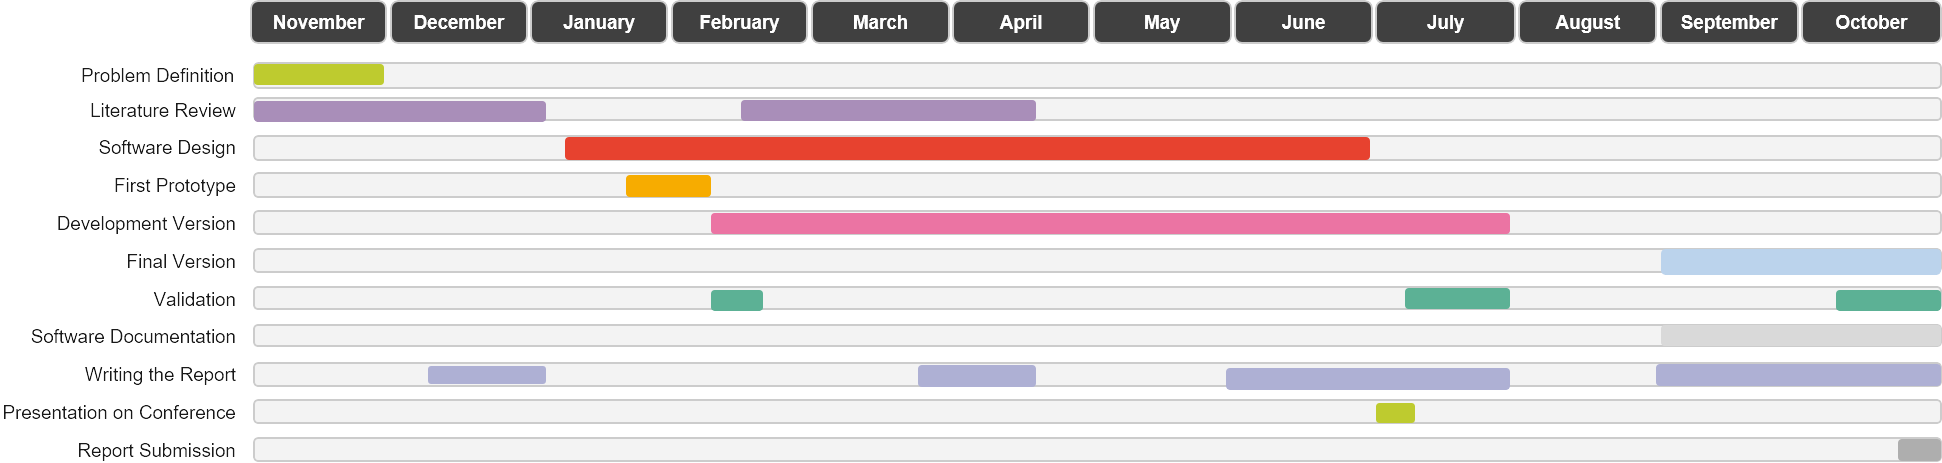
\includegraphics[width=1\textwidth]{figs/timeline2.png}
    \caption{Imagem provisória do cronograma do estágio.}
    \label{fig:timeline}
\end{figure}

\section{Theoretical Framework - Genetics and Genomics} \label{sec:intro_theoretical}
\subsection{Evolution of genetics over the years} \label{subsec:genetics_evolution}

The history of genetics formally began in 1865 with Gregor Mendel's work on plant hybridization. However, the term "genetics" was only coined in 1906 by the English biologist William Bateson to define the new science of heredity. Based on Mendel's laws, genetics introduced groundbreaking concepts such as gene, genotype, and phenotype. By the 1910s, Mendelian genetics merged with the chromosomal theory of inheritance, giving rise to classical genetics. In this framework, the gene was seen as a unit of function, transmission, recombination, and mutation. \cite{genetictimeline2}

This understanding persisted until the 1950s, when \ac{dna} was discovered as the material basis of heredity, marking the start of molecular biology. \cite{Gayon2016}

Following the discovery of \ac{dna} as hereditary material, molecular biology began to uncover the complexity of gene function. The fusion of Mendel's ideas with chromosomal theory also provided a more tangible understanding of genes, which could now be physically located on chromosomes. This integration led to significant advances, such as explaining Mendel's laws through cellular mechanisms and discovering genetic recombination. Genetics evolved into a more institutionalized science, with the establishment of academic chairs and specialized courses worldwide, solidifying its position as a central field in the biological sciences. \cite{Gayon2016}

The emergence of genomics in the latter half of the 20th century further transformed the field of genetics. The completion of the \ac{hgp} in 2003 \cite{Collins1995}, a milestone in genomics, revealed the entire sequence of human \ac{dna}, propelling the study of genes beyond individual units to entire genomes. This large-scale approach allowed scientists to explore the intricate network of genes and their interactions, significantly advancing our understanding of complex traits and diseases. Genomics also facilitated the development of personalized medicine, where treatments could be tailored based on an individual's genetic makeup. \cite{Gayon2016}

The discovery of the \ac{rna}-guided CRISPR-Cas9 system has made genome editing easier and more efficient. This breakthrough allows scientists to modify \ac{dna} in various cells and organisms with ease, removing previous experimental barriers. Today, CRISPR-Cas9 is widely used in basic research, biotechnology, and the development of new therapies. \cite{CRISPR-CAS9}

Figure \ref{fig:timeline} presents a timeline with some of the major historical milestones in the evolution of genetics over the years.

\begin{figure}[H]
    \centering
    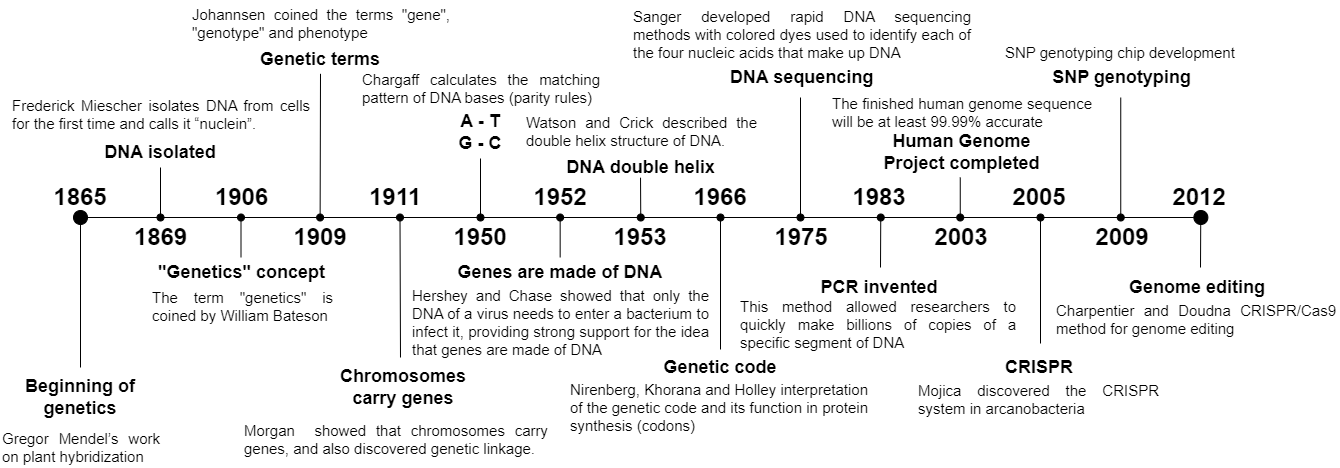
\includegraphics[width=1\textwidth]{figs/timeline.png}
    \caption{Evolution of genetics over the years: A brief timeline with some of the major historical milestones. Image adapted from \cite{genetictimeline} and \cite{genetictimeline2}}
    \label{fig:timeline}
\end{figure}

\subsection{Genetics vs Genomics} \label{subsec:genetics_genomics}

Genetics and genomics are both fields of study that explore the roles of genes in living organisms, but they focus on different aspects of heredity and \ac{dna}. Genetics is the study of specific genes and their influence on traits and conditions that are passed from one generation to the next. It examines how certain genes cause inherited disorders, such as cystic fibrosis and Huntington's disease. \cite{NHGRI2018}

In contrast, genomics is a more recent field that encompasses the study of all the genes within an organism, referred to as the genome, and how these genes interact with each other and the environment. Unlike genetics, which focuses on individual genes, genomics uses advanced technologies like bioinformatics and high-performance computing to analyze vast amounts of genetic data. This comprehensive approach is crucial for studying complex diseases, such as cancer and diabetes, which result from the interplay between multiple genes and environmental factors. While both fields contribute to advancements in health and disease treatment, genomics represents a broader, more holistic view of genetic influence. \cite{JAX2017}

\subsection{Structure and function of \acs{dna}, \acs{rna}, and proteins} \label{subsec:genetics_structure}

Nucleic acids, specifically  \ac{dna} and \ac{rna}, are fundamental molecules in biological systems, playing key roles in storing and transmitting genetic information. \ac{dna}, which exists primarily as a double-stranded helix, encodes the instructions necessary for the growth, development, and reproduction of all living organisms. \ac{rna}, on the other hand, serves multiple purposes, including acting as a messenger that carries genetic information from \ac{dna} to the ribosomes for protein synthesis. The structural complexity and functional versatility of these molecules underscore their importance in the central dogma of molecular biology, which describes the flow of genetic information from \ac{dna} to \ac{rna} to proteins. \cite{Minchin2019}

\subsection{Molecular Structure of \acs{dna}} \label{subsec:genetics_molecular}

The molecular structure of \ac{dna} is a polymer composed of repeating units called nucleotides. Each nucleotide consists of three components: a five-carbon sugar (deoxyribose), a phosphate group, and a nitrogenous base. The nitrogenous bases are categorized into two groups: purines (adenine and guanine) and pyrimidines (cytosine and thymine). The nucleotides are linked together by phosphodiester bonds, forming a sugar-phosphate backbone that gives \ac{dna} its structural integrity. \ac{dna} molecules are double-stranded, with two complementary strands running in opposite directions (antiparallel orientation). These strands are held together by hydrogen bonds between specific base pairs: adenine pairs with thymine, and guanine pairs with cytosine. This complementary base pairing is crucial for the accurate replication and transmission of genetic information. \cite{Minchin2019}

The Figure \ref{fig:dna} shows a representation of the molecular structure of \ac{dna} and the base pairing between adenine (A), thymine (T), cytosine (C), and guanine (G).

\begin{figure}[H]
    \centering
    \includegraphics[width=1\textwidth]{figs/dna.png}
    \caption{Representation of \ac{dna} and its constituents. In the top left corner, the nitrogenous bases are illustrated, categorized into Purines (Guanine and Adenine) and Pyrimidines (Thymine and Cytosine). Below this, on the left side, the paired nitrogenous bases are shown, along with their respective hydrogen bonds and the sugar-phosphate backbone connections. On the right side of the image, a chromosome is depicted unraveling, revealing the \ac{dna} structure. \cite{DNA}} 
    \label{fig:dna}
\end{figure}

\subsection{Discovery of the Double Helix} \label{subsec:genetics_discovery}

The three-dimensional structure of \ac{dna}, famously known as the double helix, was elucidated by James Watson and Francis Crick in 1953. Their discovery was informed by Rosalind Franklin’s X-ray diffraction images, which revealed the helical structure of \ac{dna}. Watson and Crick proposed that the two strands of the helix are wound around each other, with the sugar-phosphate backbone on the outside and the nitrogenous bases on the inside. The helical structure is right-handed, with ten base pairs per turn of the helix. The stability of the double helix is largely due to the hydrogen bonds between the complementary base pairs and the hydrophobic interactions between the stacked bases. This discovery not only explained how \ac{dna} could carry genetic information but also provided insights into how it could be replicated during cell division. \cite{Minchin2019}

\begin{figure}[H]
\centering
\begin{subfigure}{.5\textwidth}
    \centering
    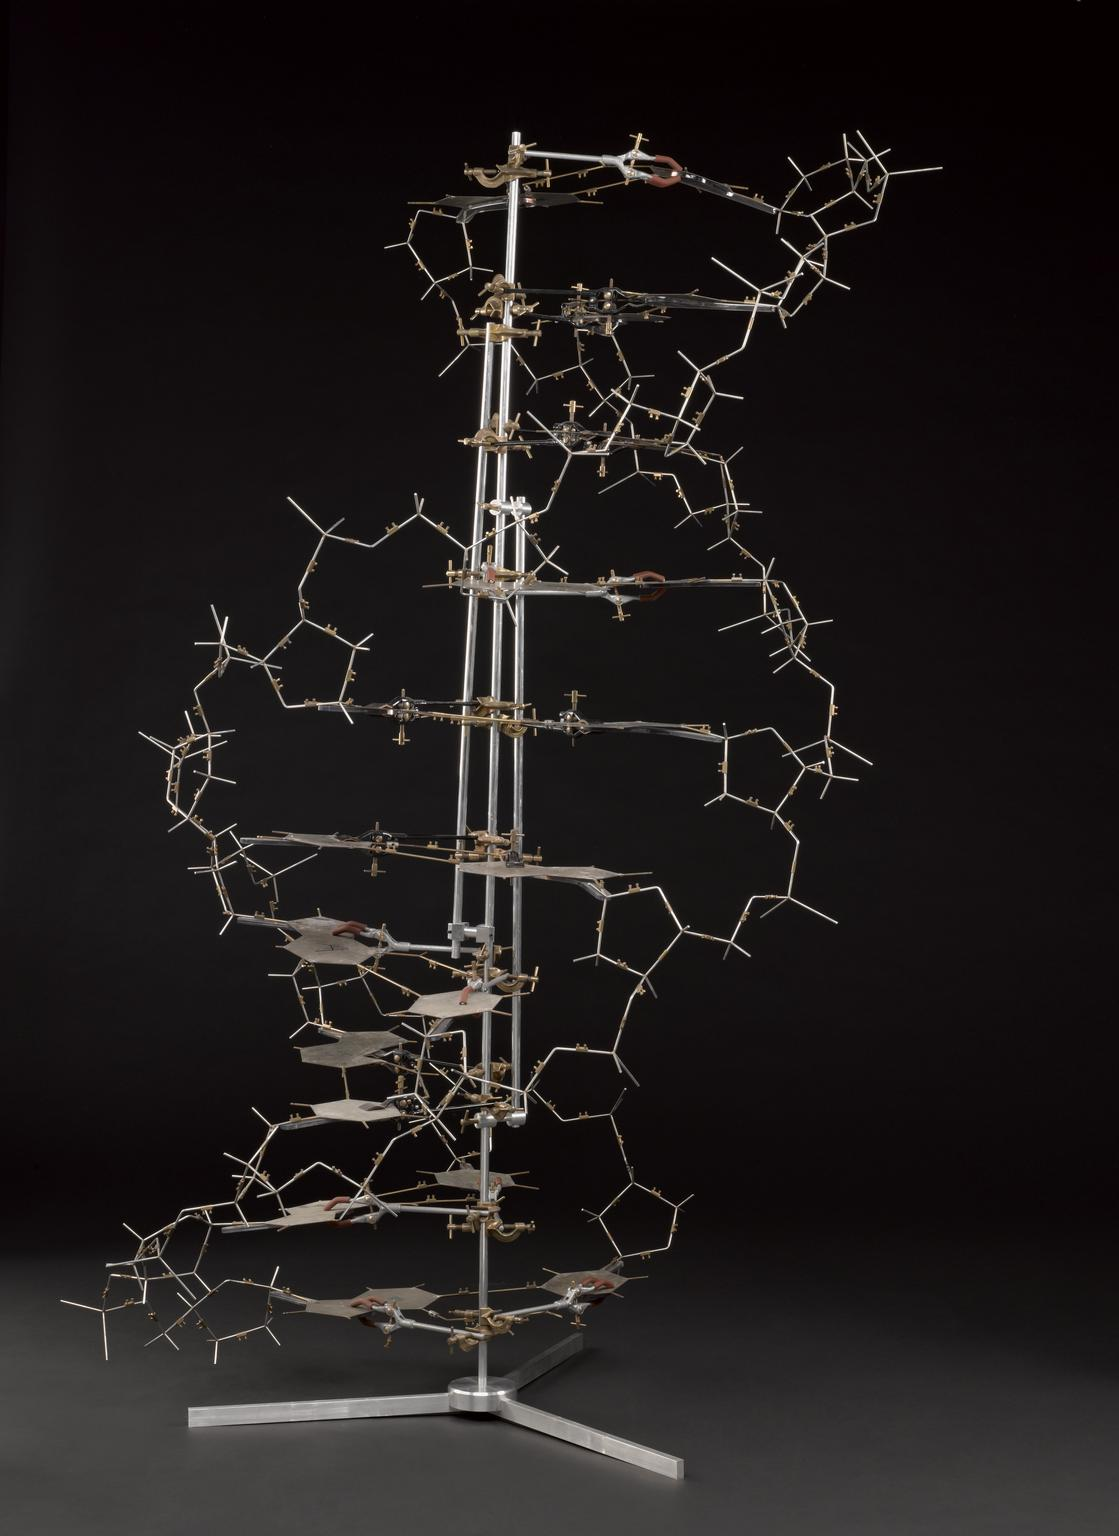
\includegraphics[width=.4\linewidth]{figs/watson_crick.jpg}
    \caption{Double helix model of \ac{dna}}
    \label{fig:watcrick}
\end{subfigure}%
\begin{subfigure}{.5\textwidth}
    \centering
    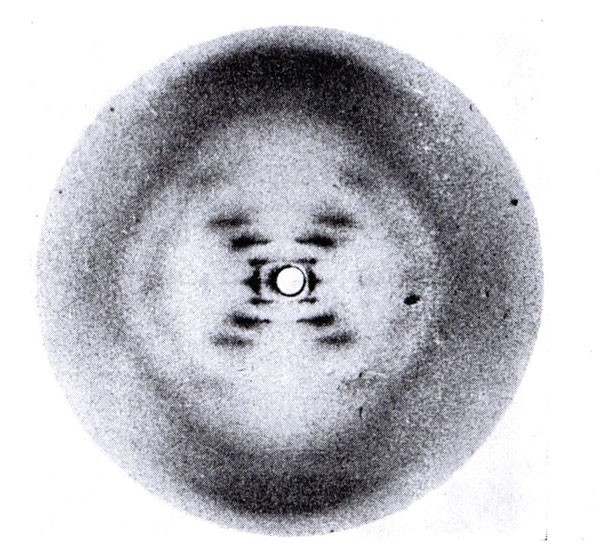
\includegraphics[width=.6\linewidth]{figs/franklin.jpg}
    \caption{X-ray diagram of \ac{dna}}
    \label{fig:franklin}
\end{subfigure}
\caption{A figure with the reconstruction of the Watson-Crick's double helix model of \ac{dna} in \ref{fig:watcrick} built by Science Museum Group Collection \cite{watcrick} and Franklin's X-ray diagram of the B form of sodium thymonucleate (\ac{dna}) fibres in \ref{fig:franklin}, published in Nature on 25 April 1953 \cite{Maddox2003}}
\label{fig:test}
\end{figure}


\subsection{\acs{dna} Packaging in Eukaryotic Cells} \label{subsec:genetics_packaging}

In eukaryotic cells, \ac{dna} is not free-floating within the nucleus; instead, it is highly organized and compacted into structures known as chromosomes. This compaction is achieved through the association of \ac{dna} with histone proteins, forming nucleosomes, which are the basic unit of chromatin. Each nucleosome consists of a segment of \ac{dna} wrapped around a core of histone proteins. These nucleosomes are further coiled and folded into higher-order structures, eventually forming the condensed chromosomes visible during cell division. The packaging of \ac{dna} into chromatin is essential for fitting the large eukaryotic genome into the limited space of the nucleus. Furthermore, chromatin structure plays a crucial role in gene regulation, as regions of tightly packed chromatin (heterochromatin) are generally transcriptionally inactive, while loosely packed regions (euchromatin) are more accessible to transcriptional machinery. \cite{Minchin2019}

\subsection{Mutations and genetic variations} \label{subsec:genetics_mutations}

Mutations are fundamental drivers of genetic diversity, occurring when changes happen in the \ac{dna} sequence. These alterations can range from small-scale mutations, such as the substitution, insertion, or deletion of one or a few nucleotides, to large-scale mutations that involve significant chromosome segments or entire genes. Chromosome mutations specifically impact either individual nucleotides or larger chromosome fragments. They can involve deletions, insertions, inversions, translocations, or even gene duplications. On the other hand, genome mutations refer to changes in the number of whole chromosomes or sets of chromosomes and are studied separately. \cite{merrick2016}

Genetic variation, on the other hand, refers to the observable differences between individuals within a population, which arise from variations in their genotypes. While mutations are the source of new genetic variation, genetic variation encompasses the broader concept of how different alleles at specific loci contribute to diversity within a population. This variation is shaped and refined by evolutionary forces such as natural selection, gene flow, and genetic drift. In cultivated plants, human-directed selection can also manipulate genetic variation to enhance desirable traits. \cite{merrick2016}

\section{Theoretical Framework - Sequencing Methods and Characteristics} \label{sec:intro_sequencing}

Even though there are several methods for sequencing \ac{dna}, the most widely used technique nowadays is \acl{ngs}. This section focuses only on \ac{ngs} and its applications, including gene panels, exome sequencing, and genome sequencing.

\subsection{\acl{ngs} - Gene Panels, Exome, and Genome Sequencing} \label{subsec:ngs_gp_es_gs}


\acl{ngs} technologies have revolutionized genomic medicine, enabling rapid advancements in clinical diagnostics, therapeutic decision-making, and disease prediction. Unlike traditional sequencing methods such as Sanger sequencing, which are limited by low throughput and high cost \cite{cost}, \ac{ngs} allows for the massively parallel sequencing of \ac{dna}, significantly increasing throughput and reducing costs by several orders of magnitude. As a result, clinical laboratories now have the capability to analyze nearly complete exomes or genomes of individuals, thereby improving the diagnostic process for a wide range of genetic conditions. \cite{Rehm2013}

\ac{ngs} is characterized by the use of clonally amplified or single molecule templates, which are sequenced in parallel, providing an unprecedented ability to analyze large amounts of \ac{dna} efficiently. The adoption of \ac{ngs} in clinical settings is growing rapidly, with three primary applications gaining prominence: disease-targeted gene panels, \ac{es}, and \ac{gs}. \cite{Rehm2013}

\subsubsection{\textbf{Disease-targeted gene panels}} \label{subsubsubsec:ngs_panels}

Disease-targeted gene panels focus on a set of known disease-associated genes, allowing for greater depth of coverage and increased analytical sensitivity. This targeted approach improves the detection of heterozygous variants, mosaicism, or low-level heterogeneity, particularly in applications related to mitochondrial diseases or oncology. Targeted panels also allow laboratories to leverage desktop sequencers, reducing the costs of sequencing and data storage. However, follow-up techniques such as Sanger sequencing may be required to fill gaps in the data caused by regions of low coverage. \cite{Rehm2013}

\subsubsection{\textbf{\acl{es}}} \label{subsubsubsec:ngs_es}

\acl{es} targets the coding regions of the genome, which constitute approximately 1-2\% of the entire genome but harbor around 85\% of known disease-causing mutations. \cite{Majewski580} \ac{es} is particularly valuable in "detecting variants in known disease-associated genes as well as for the discovery of novel gene-disease associations" \cite{Rehm2013}, with clinical studies demonstrating a diagnostic success rate of approximately 20\%. \cite{schork_genetic_2013} Despite this potential, \ac{es} faces challenges related to coverage variability, as certain exonic regions may not be captured or sequenced with sufficient depth to make a sequence call, leading to the need for additional sequencing techniques to confirm findings. \cite{Rehm2013}

\subsubsection{\textbf{\acl{gs}}} \label{subsubsubsec:ngs_gs}

\acl{gs} offers a more comprehensive approach by covering both coding and non-coding regions of the genome. This technique simplifies the preparation of samples for sequencing by eliminating the need for pre-sequencing enrichment strategies. While \ac{gs} holds promise for identifying regulatory variants and structural variants that are outside of coding regions, it remains the most expensive \ac{ngs} technology and typically provides lower average depth of coverage. Nonetheless, as technology advances, these limitations are expected to diminish, making \ac{gs} a more accessible option for clinical diagnostics. \cite{Rehm2013}

\ac{ngs} involves three major components: sample preparation, sequencing, and data analysis. These steps are interrelated, and the quality of each influences the overall outcome of the sequencing process. Below is an overview of these essential stages according to the guidelines of \cite{Rehm2013}.

\subsection{\acl{ngs} - Overview} \label{subsec:ngs_overview}

\subsubsection{\textbf{Sample preparation}} \label{subsubsec:ngs_sample}

The \ac{ngs} process begins with the extraction of genomic \ac{dna} from a biological sample, typically from a patient. The quality and quantity of this \ac{dna} are critical to successful sequencing. Laboratories must specify the required sample type and amount based on their validation data. Sample mix-ups must be prevented through robust processes, as even minor errors can significantly affect results. \cite{Rehm2013}

For specific \ac{ngs} applications like targeted panels or \ac{es}, enrichment strategies are employed to focus on a subset of genomic regions. Enrichment ensures that only the regions of interest are sequenced, improving efficiency and reducing costs. Enrichment can be achieved through various methods, including multiplex PCR and hybridization-based capture. \cite{Rehm2013}

\subsubsection{\textbf{Library Generation and Barcoding}} \label{subsubsec:ngs_library}

Library generation is the process of preparing \ac{dna} fragments of a specific size (100-500 base pairs) for sequencing. These fragments are tagged with adapter sequences on both ends, which are essential for downstream sequencing steps. The fragmentation of \ac{dna} can be performed using different methods, each with its advantages and limitations. In most \ac{ngs} workflows, PCR amplification is used to amplify the \ac{dna} library before sequencing. \cite{Rehm2013}

Barcoding is a crucial step in library preparation, where each sample is tagged with a unique sequence identifier. This allows multiple samples to be pooled together in a single sequencing run, reducing the cost per sample. Barcoding is typically integrated into the adapter sequences or added during a PCR enrichment step. \cite{Rehm2013}

\subsubsection{\textbf{Target Enrichment}} \label{subsubsec:ngs_enrichment}

In many \ac{ngs} applications, particularly targeted panels and \ac{es}, only specific regions of the genome are sequenced. Target enrichment methods are used to isolate these regions before sequencing. Target enrichment strategies include PCR-based methods (e.g., single or multiplex PCR) and hybridization-based capture. While PCR-based methods are suitable for smaller panels, hybridization-based approaches are preferred for larger-scale applications like exome sequencing. \cite{Rehm2013}

\subsubsection{\textbf{Sequencing Platforms}} \label{subsubsec:ngs_platforms}

\ac{ngs} platforms are designed to perform millions of parallel chemical reactions, allowing them to sequence vast amounts of \ac{dna} simultaneously. These platforms utilize different sequencing chemistries, such as sequencing by synthesis, sequencing by ligation, and ion sensing. \cite{glenn2011} The choice of sequencing platform depends on various factors, including sequence capacity, read length, run time, cost, and accuracy. \cite{Rehm2013}

Each platform has its own strengths and weaknesses. For example, some platforms excel at producing longer reads, while others are optimized for high-throughput sequencing at a lower cost per sample. The selection of a platform is influenced by the specific clinical or research application. \cite{Rehm2013}


\section{Theoretical Framework - Bioinformatics} \label{sec:intro_bioinformatics}

\subsection{\acl{ngs} - Data Analysis} \label{subsec:ngs_data_analysis}

\ac{ngs} generates an enormous amount of sequence data, necessitating the development of sophisticated data analysis pipelines. These pipelines are designed to process and interpret the raw sequencing data, transforming it into meaningful genomic information. \ac{ngs} data analysis can be divided into four primary steps: Base Calling, Read Alignment, Variant Calling, and Variant Annotation. The bioinformatics analysis stage of \ac{ngs} is essential for converting unprocessed sequencing data into biologically and clinically significant findings. This section provides a bioinformatics overview of these steps and their importance in the \ac{ngs} workflow. \cite{Rehm2013}

\subsubsection{\textbf{Base Calling}} \label{subsubsec:ngs_basecalling}

Finding the nucleotide at each place in a sequencing read is known as \textbf{Base Calling}. In order to ensure that the raw data gathered during sequencing is transformed into a sequence of nucleotides, this step is usually included into the software of the sequencing device. \cite{Rehm2013} 

For example, the Illumina NovaSeq 6000 Sequencing System uses two-channel sequencing approach, requiring only two images to represent data for all four \ac{dna} bases, with one image capturing information from the red channel and the other from the green channel. \cite{NovaSeq}

An 'N' designation, or 'no call' is used when a cluster fails to meet quality filters, registration is unsuccessful, or the cluster is not properly captured in the image. The process involves extracting intensity data for each cluster from both the red and green images and comparing these intensities to identify four distinct populations. Each of these populations is associated with one of the \ac{dna} bases, and the base calling process assigns each cluster to the corresponding population. \cite{NovaSeq}

Figure \ref{fig:cluster} illustrates the intensity data for each cluster from both the red and green channels in 2-channel sequencing, as used in the NovaSeq 6000 Sequencing System.

\begin{figure}[H]
    \centering
    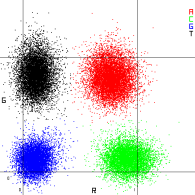
\includegraphics[width=0.3\textwidth]{figs/ClusterIntensities.png}
    \caption{Visualization of cluster intensities in 2-Channel Sequencing (NovaSeq 6000 - Illumina). The image shows the intensity data for each cluster from both the red and green channels, with each cluster representing a different \ac{dna} base. Image from \cite{NovaSeq}.} 
    \label{fig:cluster}
\end{figure}

Table \ref{tab:base_call} outlines how the signal intensities from red and green fluorescence channels are used to identify \ac{dna} bases (A, C, G, T) during sequencing. Each base is associated with a unique combination of signal intensities from these two channels. The red and green channels either show intensity, marked as "on" (1), or no intensity, marked as "off" (0), at specific cluster locations where \ac{dna} bases are being read.

When both the red and green channels show intensity (1,1), this indicates the presence of adenine (A). The simultaneous detection of both red and green signals suggests that the cluster is emitting light in both spectrums, and this combination is uniquely attributed to adenine.

For cytosine (C), the red channel is on (1), but the green channel is off (0). This means that the cluster emits light in the red spectrum only, and the absence of green emission differentiates it as cytosine.

When neither the red nor the green channel shows intensity (0,0), the system identifies guanine (G). The lack of any signal at a known cluster location suggests that no fluorescence is being emitted, and this corresponds to guanine.

Finally, thymine (T) is identified when the red channel is off (0) and the green channel is on (1). In this case, the cluster is emitting light in the green spectrum only, and the absence of red fluorescence distinguishes it as thymine.

This method of combining red and green fluorescence signals allows the sequencing system to effectively differentiate between the four \ac{dna} bases by associating specific patterns of signal intensity with each base.

\begin{table}[H]
    \centering
    \caption{Base Calls in 2-Channel Sequencing (NovaSeq 6000 - Illumina). Table from \cite{NovaSeq}}
    \label{tab:base_call}
    \resizebox{\textwidth}{!}{%
    \begin{tabular}{@{}cccl@{}}
    \toprule
    \textbf{Base} & \textbf{Red Channel} & \textbf{Green Channel} & \multicolumn{1}{c}{\textbf{Result}} \\ \midrule
    A & 1 (on)  & 1 (on)  & Clusters that show intensity in both the red and green channels. \\
    C & 1 (on)  & 0 (off) & Clusters that show intensity in the red channel only.            \\
    G & 0 (off) & 0 (off) & Clusters that show no intensity at a known cluster location.     \\
    T & 0 (off) & 1 (on)  & Clusters that show intensity in the green channel only.          \\ \bottomrule
    \end{tabular}
    }
\end{table}


\subsubsection{\textbf{Read Alignment/Mapping}} \label{subsubsec:ngs_alignment}

Base calling is followed by demultiplexing, the process of separating reads from different samples based on their unique barcodes. After demultiplexing, the next step is store reads in a FASTQ file, a text-based format that includes a read identifier, the nucleotide sequence, a separator, and a quality score string. The quality scores are calculated using the Phred scale, which represents the likelihood of a base call being correct, with higher scores indicating greater confidence. For a given base error probability, P, the Phred quality score, Q, is calculated in Equation \ref{eq:phred}.

\begin{equation}\label{eq:phred}
    Q = -10 \log_{10} P
\end{equation}

FASTQ is the standard format for raw sequencing data and is commonly used in single-end and paired-end sequencing. \cite{Larson2023} The Figure \ref{fig:fastq} shows an example of a FASTQ file, with the read identifier, nucleotide sequence, and quality score (highlighting the score for one T base and the respective P error).

\begin{figure}[H]
    \centering
    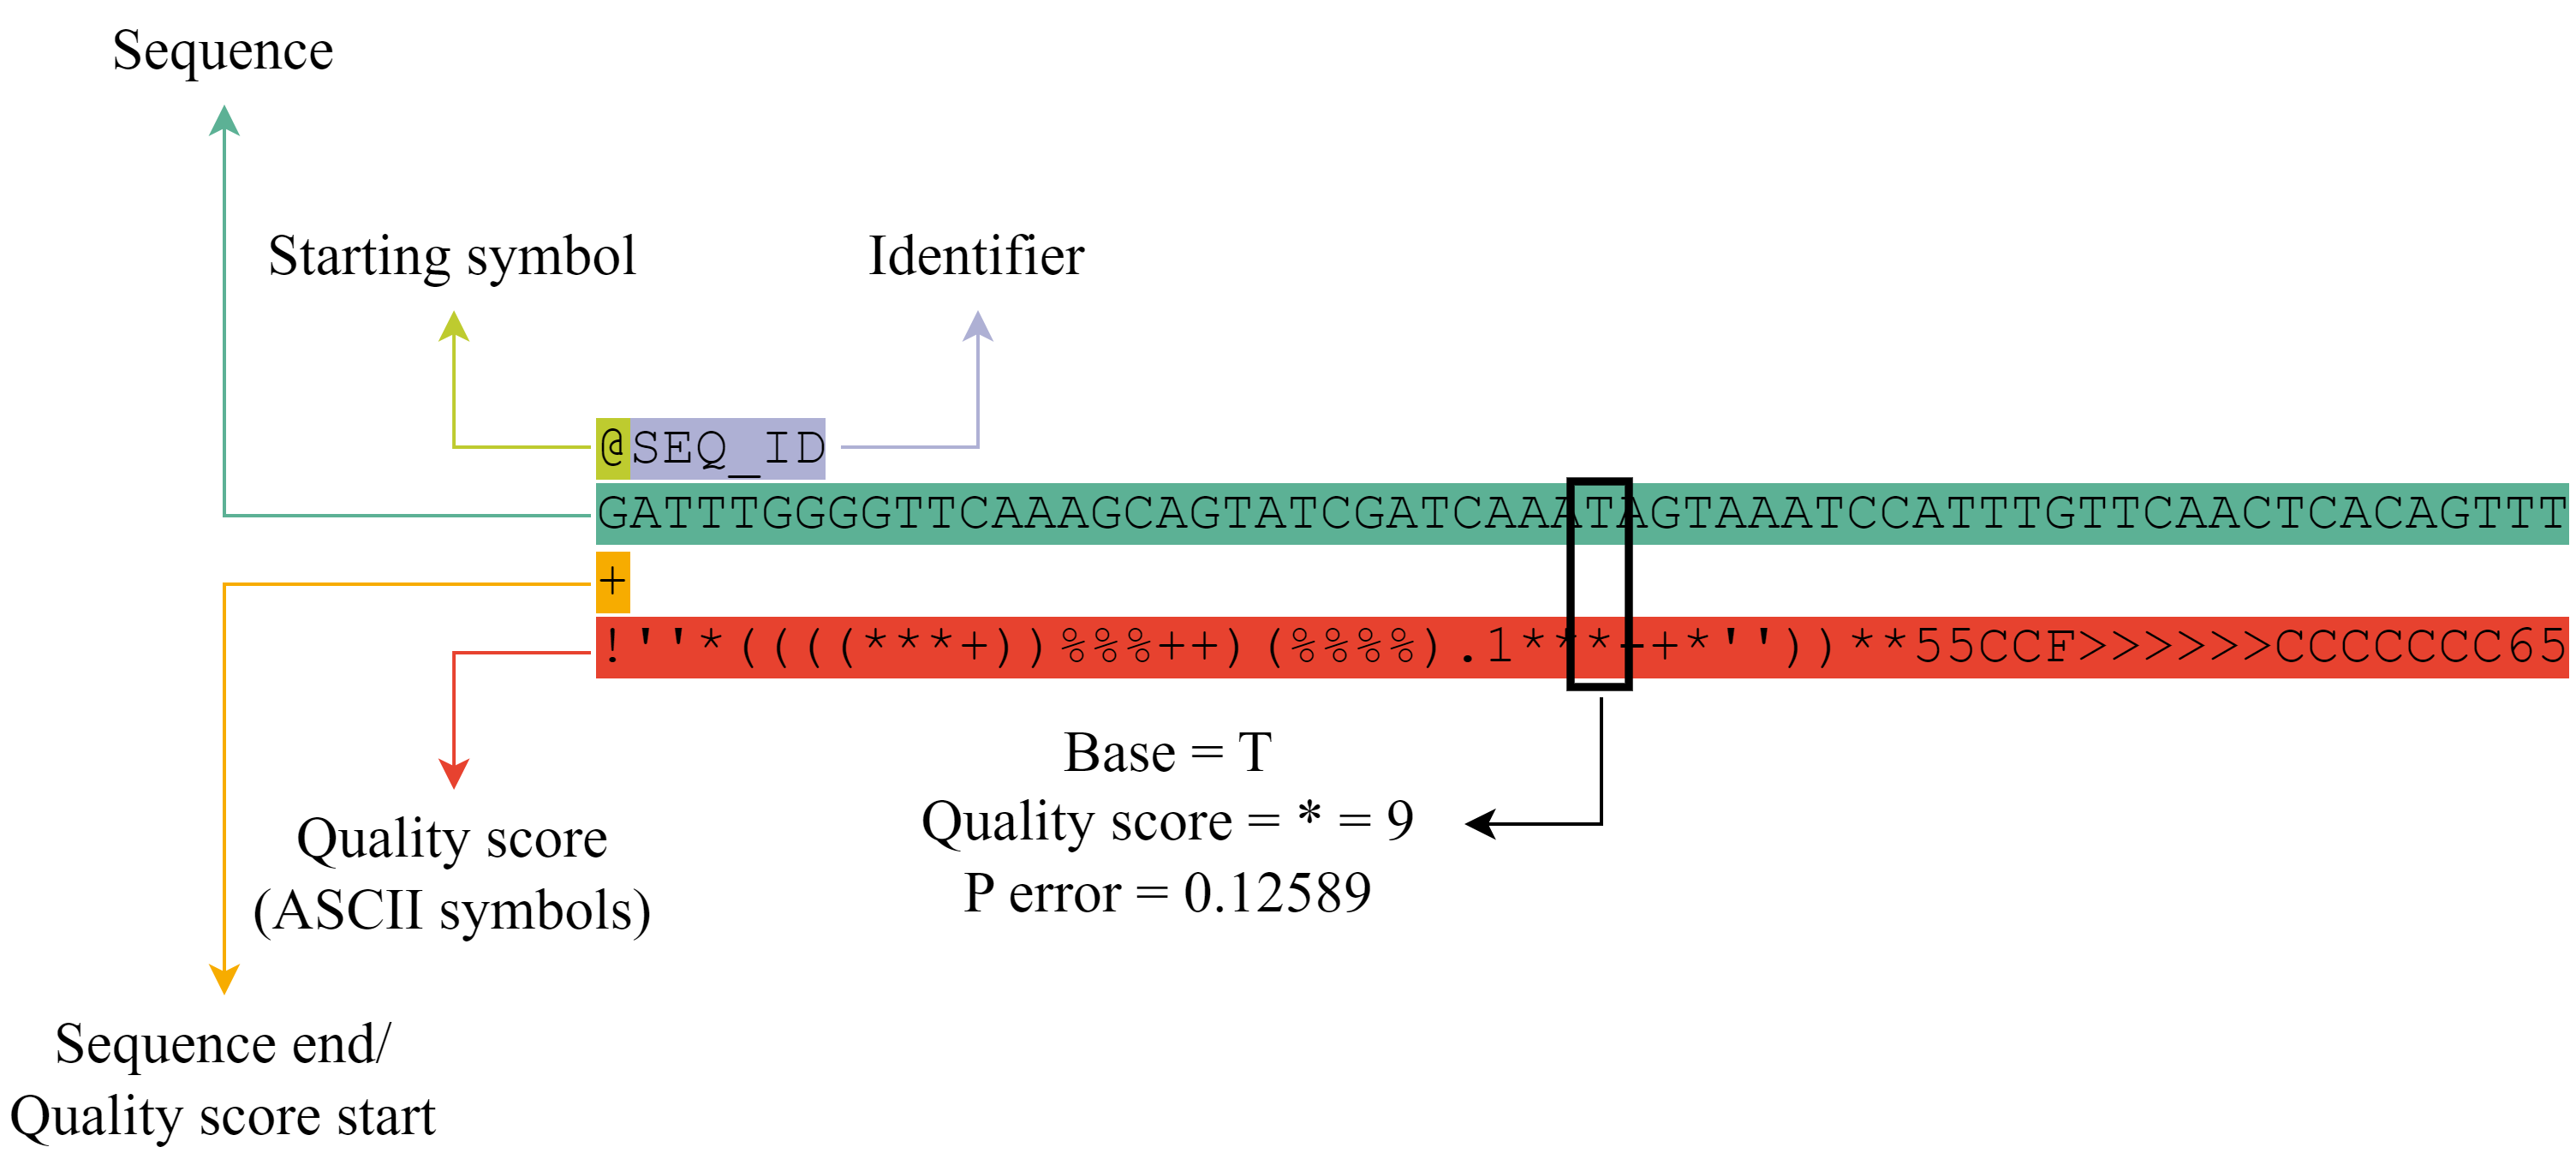
\includegraphics[width=1\textwidth]{figs/fastq.png}
    \caption{FASTQ file format example. The image shows a read identifier, nucleotide sequence, and quality score string in a FASTQ file. The P error calculation was performed based on the Phred quality score equation and Quality Score Encoding from Table \ref{tab:fastq_encoding}. This file example was adapted from \cite{Wikipedia2024}.} 
    \label{fig:fastq}
\end{figure}

Once the raw sequencing data was stored in a FASTQ file, the next step is \textbf{Read Alignment/Mapping}. \cite{Larson2023} In this stage, the small \ac{dna} sequences (50–400 base pairs), reads, are positioned in relation to a reference genome, such as \ac{hg38}.  \cite{Rehm2013} To improve alignment accuracy, low-quality bases and adapter sequences are also trimmed and the results are saved in either \ac{sam} or \ac{bam} formats, with \ac{bam} being more efficient due to compression and indexing capabilities. A more compressed format, \ac{cram}, further reduces file sizes by storing only differences from the reference genome, though it uses lossy compression in some cases (meaning that some \ac{cram} files may not be fully convertible back to \ac{bam}) \ac{cram} is becoming a popular choice for long-term data storage due to its space efficiency - a \ac{cram} file could be 50\%-80\% smaller than a \ac{bam} file. \cite{Larson2023}

\subsubsection{\textbf{Variant Calling}} \label{subsubsec:ngs_variantcalling}

\textbf{Variant Calling} identifies genetic differences between a sample's sequencing reads and a reference genome using specialized algorithms known as variant callers. Common variants, include single-nucleotide polymorphisms (SNPs), single-nucleotide variants (SNVs), small insertions and deletions (INDELs), and copy number variants or alterations (CNVs and CNAs). The first tree are related to Sequence Variants, while the last one is related to Structural Variants. \cite{Roy2018}, \cite{pipeline}, \cite{Roy2020}, \cite{Kanzi2020} SNPs refer to single-base changes in germline DNA, often biallelic, while SNVs cover any point mutation. CNVs involve larger DNA segments that are amplified or deleted, and CNAs specifically refer to somatic changes, often observed in cancer. \cite{Larson2023} There are also other types of variants, such as translocations, inversions, and complex rearrangements, which are less common but can have significant clinical implications. \cite{Roy2018}

The confidence with which variants are called depends heavily on sequencing depth and the variant allele frequency (VAF), which measures the proportion of DNA molecules in a sample that contain the variant allele. For germline heterozygous variants, where the variant is expected to appear in roughly 50\% of reads, reliable detection can typically be achieved at sequencing depths of 20X to 30X. However, somatic variants, especially in cancer samples, tend to have lower VAFs due to tumor heterogeneity and sample contamination, requiring much higher coverage for reliable detection. \cite{Larson2023}

Preprocessing of BAM files is essential before variant calling. Duplicates, originating from the same DNA fragment, must be marked to avoid skewing VAF estimates. Deduplication is recommended for whole-genome or exome sequencing but is usually skipped in PCR-based methods. Base quality scores are also recalibrated to correct systematic errors. After preprocessing, the BAM files are ready for variant detection. \cite{Larson2023}

\textbf{Germline Variant Calling} for SNVs can be done using tools like Samtools or more advanced programs like GATK HaplotypeCaller, which improve accuracy in complex regions by applying local realignments. For biallelic SNPs, the reference allele (REF) is compared to the alternate allele (ALT). Humans, being diploid, have three possible SNP genotypes: homozygous reference (REF, REF), heterozygous (REF, ALT), and homozygous alternate (ALT, ALT), corresponding to variant allele frequencies (VAFs) of 0\%, 50\%, and 100\%. Genotype quality (GQ), similar to base quality scores, reflects the confidence in a genotype call, measured on a Phred scale. \cite{Larson2023}

When detecting copy number variants (CNVs) using NGS data, algorithms primarily rely on sequencing coverage patterns, although they may also take into account the VAFs of overlapping variants. CNV detection in targeted sequencing approaches like whole-exome sequencing (WES) or gene panels can be challenging due to coverage gaps and inconsistencies caused by capture bias. As a result, CNV identification within individual samples is difficult, and many tools designed for this purpose compare the data against a reference set of normal samples. \cite{Larson2023}

\textbf{Somatic Variant Detection} is enhanced by comparing tumor and matched normal tissue sequencing data, allowing inherited germline variants to be filtered out. When matched normal samples are unavailable, a “panel of normals” can serve as a reference. Additionally, classifiers trained on databases of somatic and germline variants can help predict the somatic status of variants found in tumor tissue. Despite these approaches, somatic variant detection still faces challenges, particularly due to the Euro-centric bias of many population allele frequency databases, which may reduce the accuracy of variant calls in underrepresented populations. \cite{Larson2023}

Variants are typically stored in variant call format (VCF) files, which can include data from multiple samples. Genomic VCF (gVCF) files capture both variant and non-variant regions, allowing for easier data merging. Both VCF and gVCF files can be indexed for efficient access. Somatic mutations may also be saved in Mutation Annotation Format (MAF) files, which aggregate variant data from multiple VCFs. \cite{Larson2023}

\subsubsection{\textbf{Variant Annotation}} \label{subsubsec:ngs_annotation}
Once variants are called, \textbf{Variant Annotation} is carried out. This involves adding contextual information to each detected variant, such as determining its location within or near a gene and predicting its potential impact on protein function. Clinical interpretation of variants often includes data from variant databases, evolutionary conservation studies, and in silico predictions of pathogenicity. \cite{Rehm2013} 

\ac{ngs} often generates numerous variants, including many \ac{vus}, making it difficult to determine which are clinically relevant. Variant annotation helps prioritize and interpret these findings. For protein-coding regions, tools like REVEL \cite{REVEL} predict the functional impact of missense variants, while noncoding variants are assessed using resources such as CADD \cite{CADD}, FunSeq2 \cite{FunSeq2}, and RegulomeDB \cite{RegulomeDB}. These are complemented by data from projects like ENCODE \cite{ENCODE} and Roadmap Epigenomics \cite{REC}, and external databases like gnomAD \cite{gnomAD}, ClinVar \cite{ClinVar}, HGMD \cite{HGMD}, and COSMIC \cite{COSMIC}. Annotation software like ANNOVAR \cite{ANNOVAR} integrates these resources to enrich VCF files with variant details. \cite{Larson2023}

Overall, accurate and efficient data analysis in NGS requires significant bioinformatics support and robust computational infrastructure. This aspect of NGS is crucial for translating raw sequencing data into clinically relevant insights.

Figure \ref{fig:pipeline} illustrates the general bioinformatics analysis pipeline for NGS, highlighting the key steps mentioned previously.

\begin{figure}[H]
    \centering
    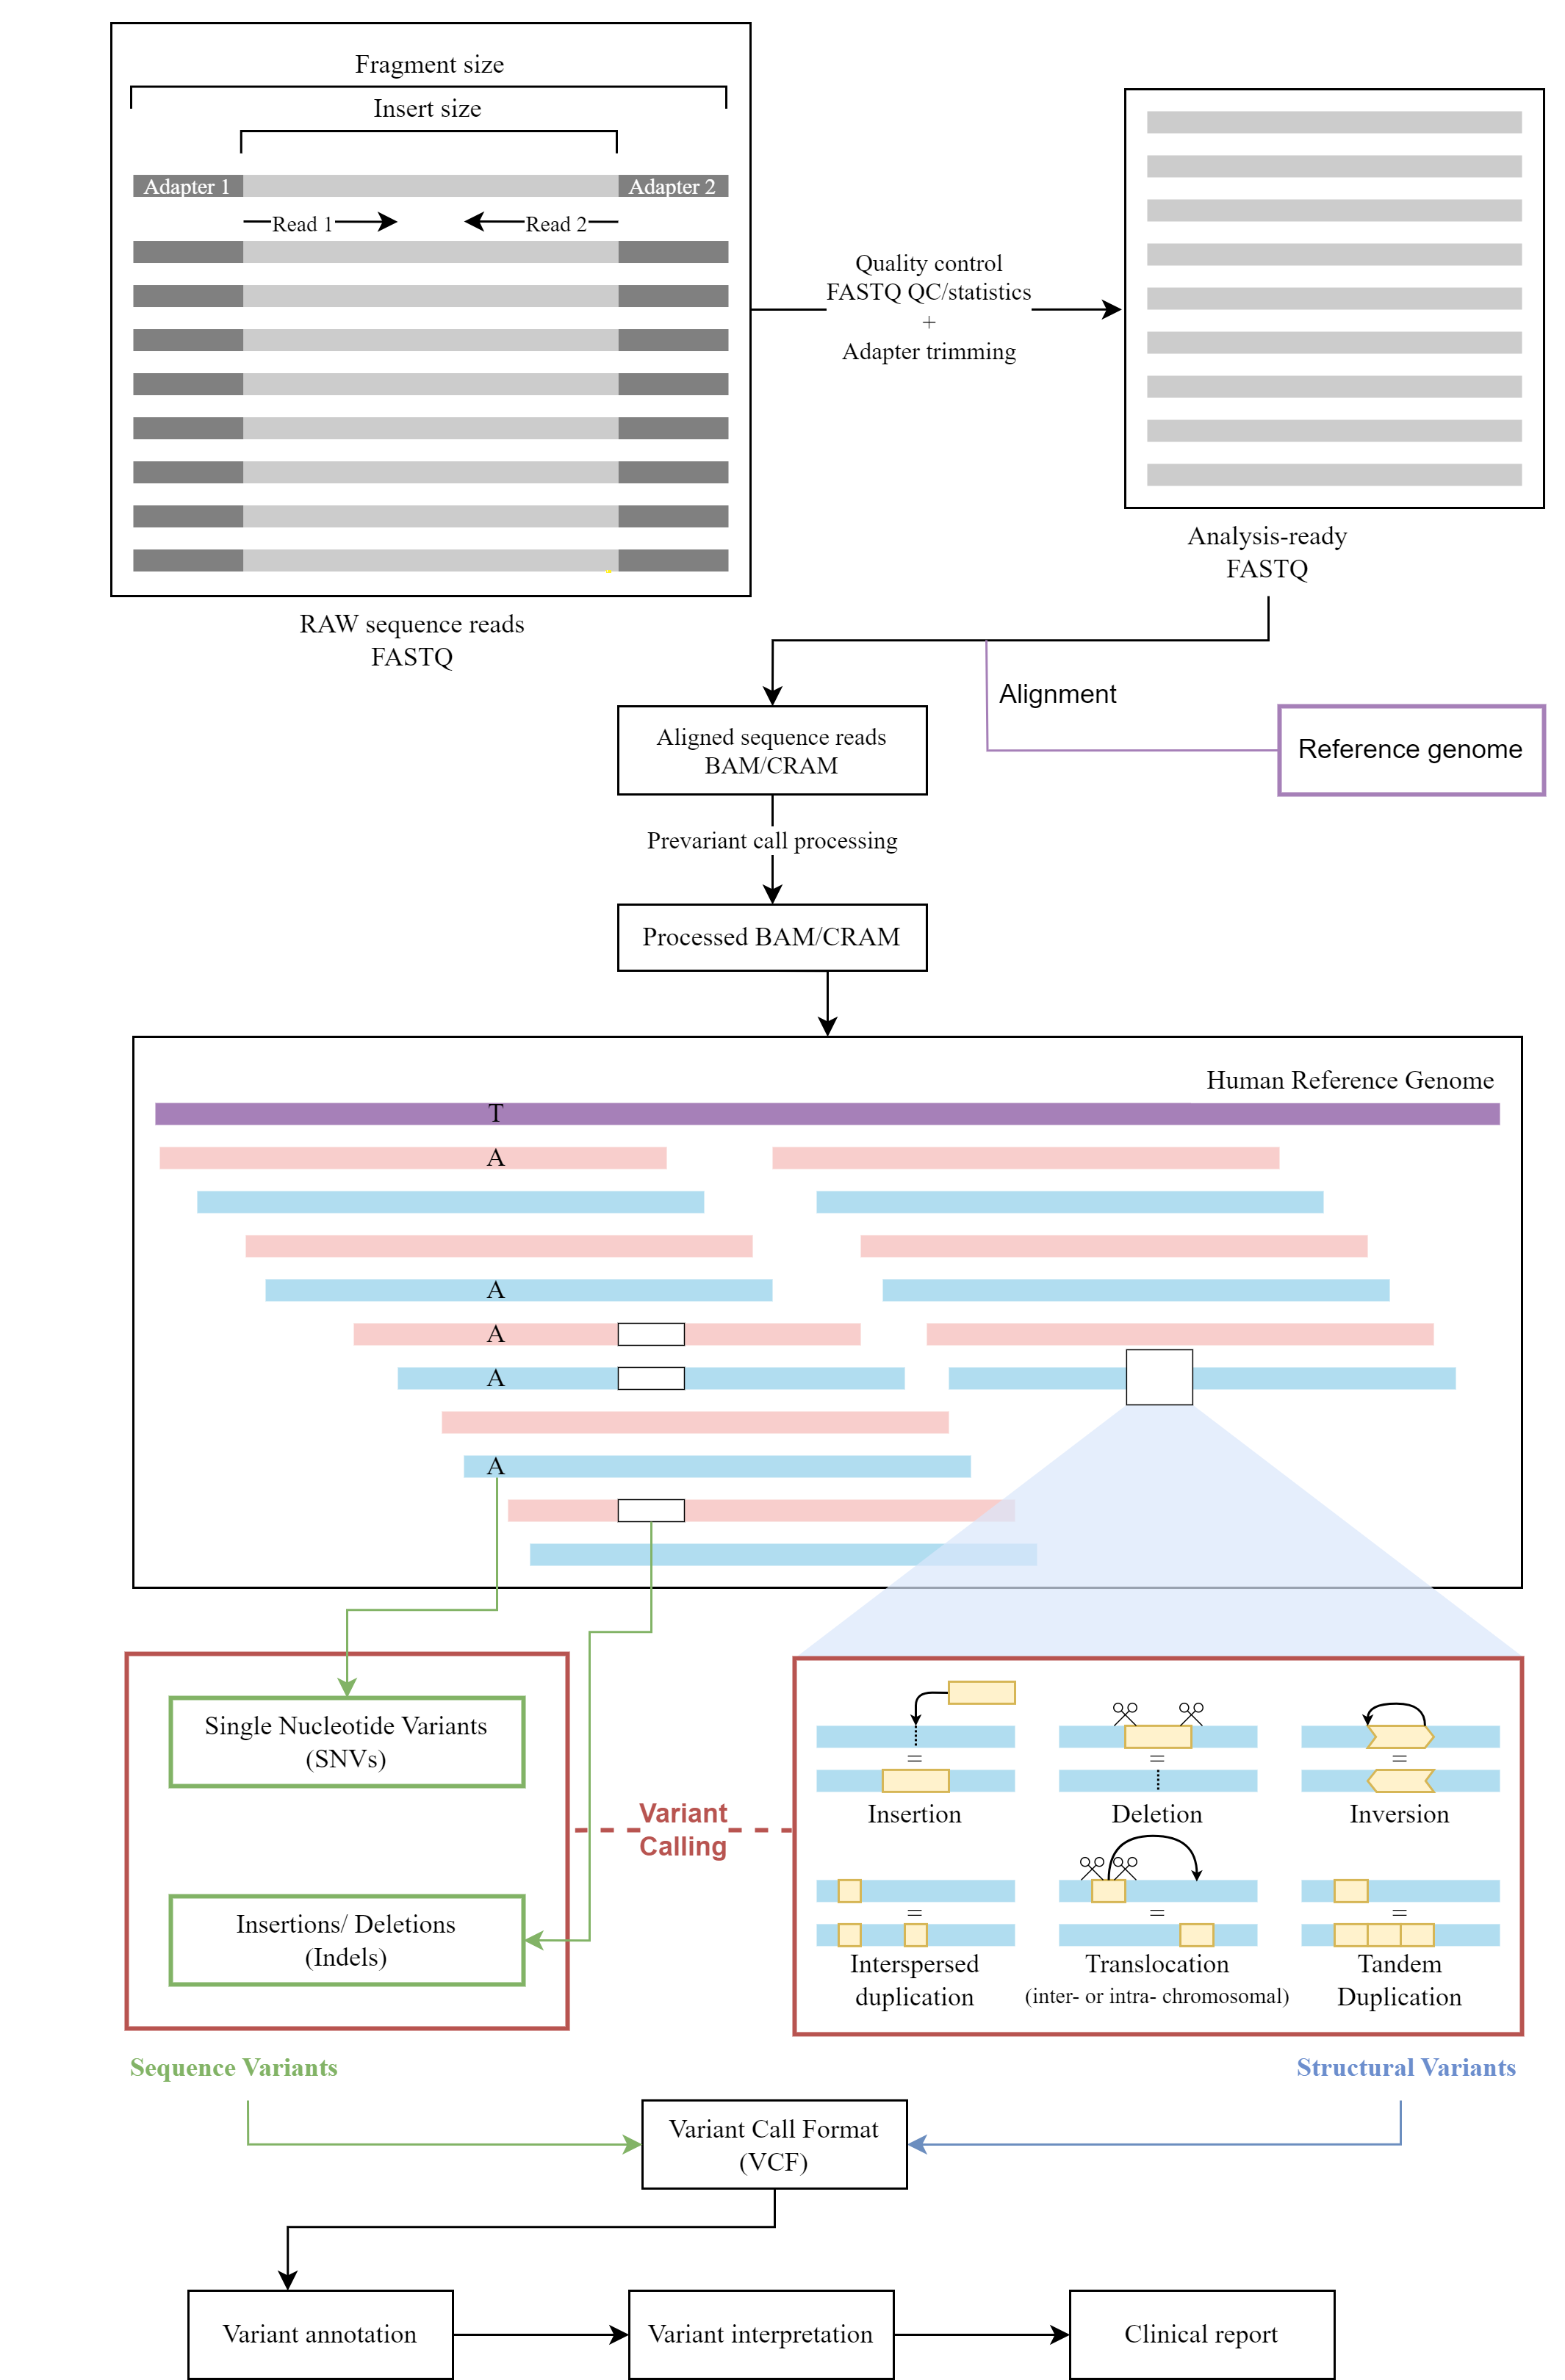
\includegraphics[width=0.9\textwidth]{figs/pipeline.png}
    \caption{NGS data analysis pipeline. Adapted from \cite{Roy2018}, \cite{pipeline}, \cite{Roy2020}, \cite{Kanzi2020}} 
    \label{fig:pipeline}
\end{figure}

\subsection{\acl{ngs} - Validation} \label{subsec:ngs_bioinformatics}

In genetic and genomic analysis, namely in \ac{ngs}, a key focus is often placed on the comparison between coverage and sequencing depth. While these terms are related, they offer distinct insights into the quality and reliability of sequencing data. A thorough understanding of both concepts is essential to ensure accurate and meaningful results in genetic studies.

\subsubsection{\textbf{Coverage or Breadth of Coverage}} \label{subsubsec:ngs_coverage}

Several elements could influence the total sequencing output, including the efficiency of the libraries, the extent of sample multiplexing, and the number of sequencing cycles. Given that the number of lanes in the flow cell is fixed, adjusting these factors is key to maximizing throughput. This throughput is commonly described in terms of coverage, which measures the proportion of the genome or target region that has been sequenced at least once. In technical documentation, coverage is often represented by a number followed by "X" such as 30X coverage. \cite{Larson2023}

Coverage focuses on ensuring that a substantial portion of the genome, or a specific target region such as the exome or a gene panel, has been adequately sequenced. It is typically expressed as a percentage. For instance, if 95\% of the intended target region has been sequenced 30X, the coverage at 30X would be expressed as "95\% coverage." However, several factors can influence coverage, including DNA sample quality, sequencing biases, and complexities within the genome, such as regions with high GC content or repetitive sequences, which can be challenging to sequence effectively. \cite{3billion2023}

Coverage is a fundamental metric in bioinformatics, as it directly impacts the reliability of detecting genetic variants. Higher coverage means that more sequencing reads overlap each base, leading to improved sensitivity and accuracy in identifying variations. In contrast, lower coverage can increase the capacity to sequence more samples or cover larger genomic areas at similar costs, although it might compromise the confidence in variant detection. \cite{Larson2023}

Different types of sequencing require varying levels of coverage. For \ac{wgs}, coverage between 30X and 50X is generally recommended, while \ac{wes} typically calls for 100X coverage. In the case of targeted gene panels, the coverage is often much greater-exceeding 500X in some cases-to ensure a high level of confidence in variant detection, particularly for somatic mutations, where greater read depth is crucial for accurate identification. \cite{Larson2023}


\subsubsection{\textbf{Sequencing/Read Depth or Depth of Coverage}} \label{subsubsec:ngs_ard}

Sequencing depth, also referred to as read depth, denotes the number of times a specific nucleotide in the DNA sequence is read during the sequencing process. It provides an indication of how thoroughly each base has been examined. The more times a nucleotide is read, the more confidence researchers can have in the accuracy of the base call, as a greater number of reads help mitigate the risk of sequencing errors and minimize noise. For instance, if a particular nucleotide is read 30 times, the sequencing depth at that location would be expressed as 30X. \cite{3billion2023}

The primary advantage of higher sequencing depth lies in its ability to enhance the precision of variant detection at specific genomic positions. This is particularly valuable when investigating rare genetic variants or when analyzing samples with significant heterogeneity, such as tumor tissues. \cite{3billion2023}

The Figure \ref{fig:depth_coverage} illustrates the relationship between coverage and depth of coverage in a gene. In this example, approximately 10\% of the gene is depicted as not covered, and the depth reaches up to 9X. This visualization highlights the importance of both coverage and read depth in ensuring the reliability of sequencing data.

\begin{figure}[H]
    \centering
    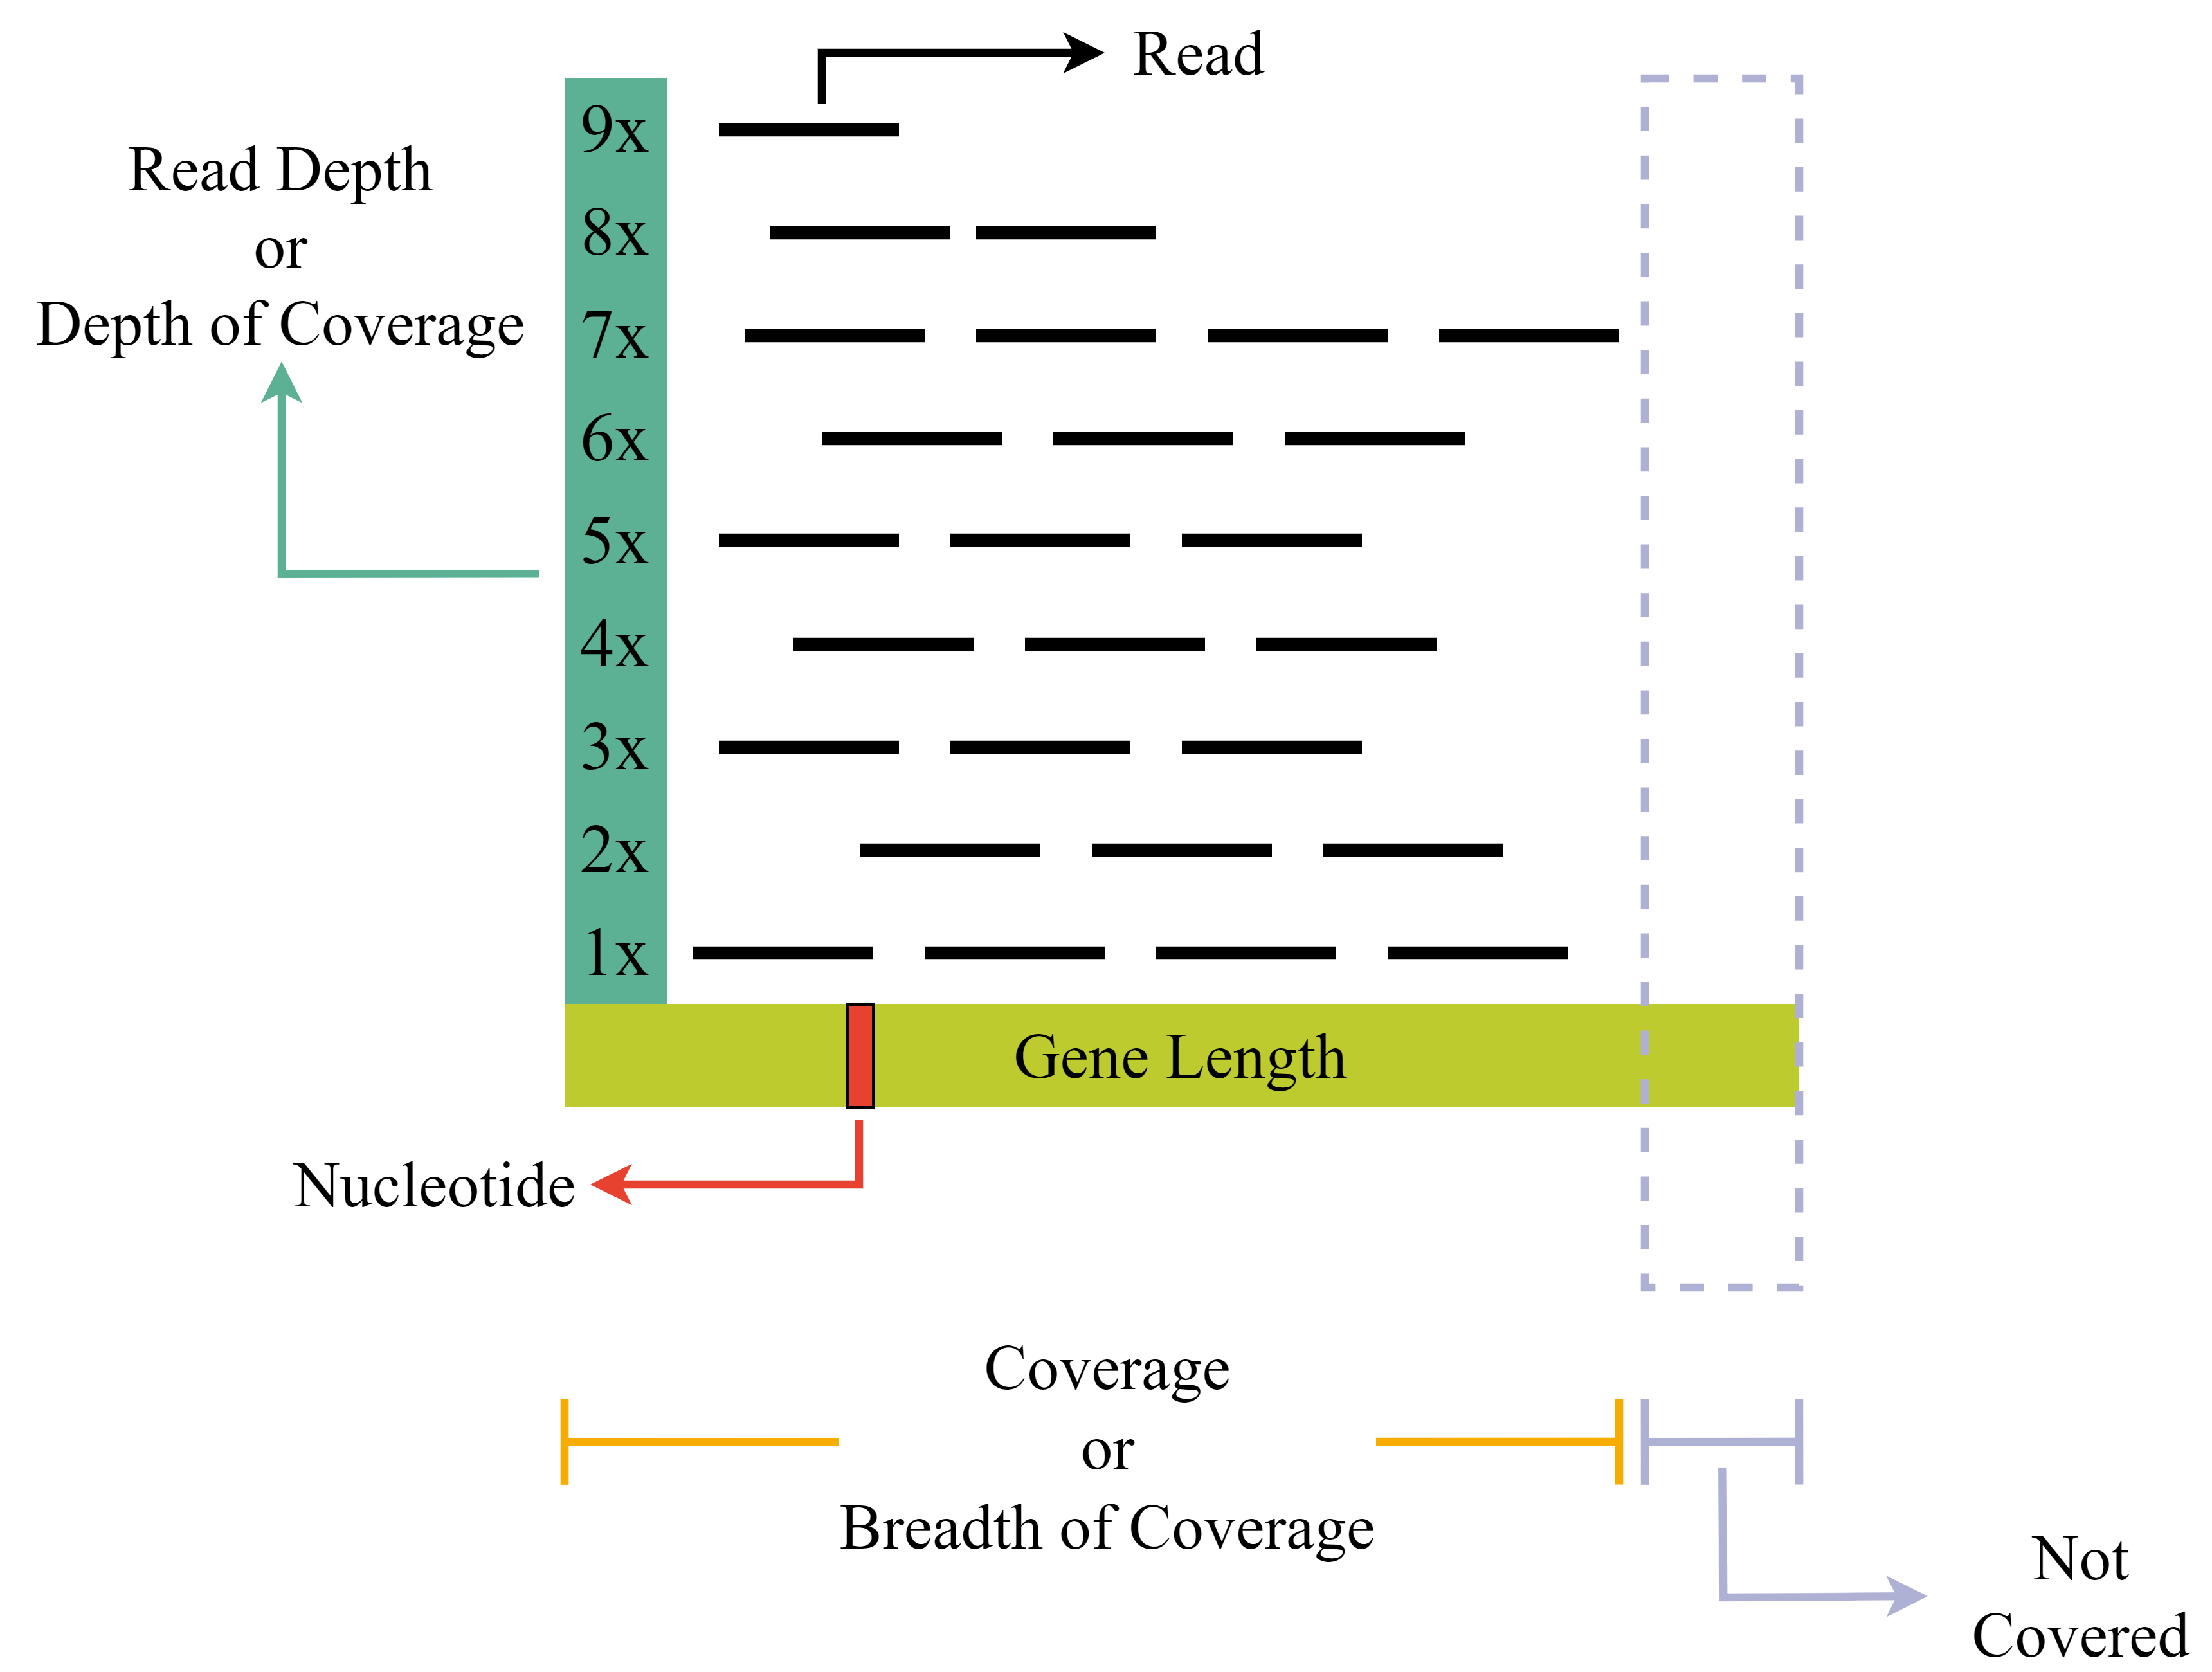
\includegraphics[width=0.8\textwidth]{figs/depth_coverage.png}
    \caption{Scheme related to Coverage/ Breadth of Coverage and Read Depth/ Depth of Coverage in a gene. In this case, approximately 10\% of the gene is depicted as not covered, and the depth reaches up to 9x. Adapted from \cite{MedGenome2020}} 
    \label{fig:depth_coverage}
\end{figure}

Given the critical importance of validation in next-generation sequencing (NGS), as previously demonstrated, this thesis focuses on the development of the following user-friendly software solution designed to calculate and ensure the accuracy of key metrics such as average read depth and coverage. These metrics are essential for evaluating the quality and reliability of sequencing data. The software presented here not only automates these calculations but also provides a streamlined and accessible interface, making it easier for users to perform NGS validation processes with consistency and precision.



